\documentclass[11pt]{article}
\usepackage[margin=1in]{geometry}

% Core packages
\usepackage{amsmath,amssymb}
\usepackage{graphicx}
\usepackage{tikz-cd}
\usepackage{multicol}

\usepackage{array}
\usepackage{tabularx}
\usepackage{booktabs}
\usepackage{xcolor}
% Language
\usepackage[spanish,es-nodecimaldot]{babel}

\usepackage[hidelinks]{hyperref}

% Secciones con la letra de la guía (A, B, C...); subsecciones A.1, A.2...
\renewcommand{\thesection}{\Alph{section}}

% Paragraphs
\setlength{\parindent}{0pt}
\setlength{\parskip}{1\baselineskip}

\begin{document}
\begin{titlepage}
    \begingroup
    \centering
    \setlength{\parskip}{0pt}

    \vspace*{1cm}
    \noindent
    \begin{minipage}[c]{0.45\textwidth}
       \centering
       \includegraphics[width=5.2cm]{UCR_logo.png}
    \end{minipage}
    \hfill
    \begin{minipage}[c]{0.45\textwidth}
       \centering
       \includegraphics[width=5.2cm]{emat_logo.png}
    \end{minipage}

    \par\vspace{1.2cm}

    {\textbf{Universidad de Costa Rica}\\[0.15cm]
    Escuela de Matemática\\[0.15cm]
    Departamento de Ciencias Actuariales\\[0.15cm]
    CA0309 Contingencias de vida II\par}

    \vspace{1.5cm}

    {\textbf{Proyecto Final}\par}

    \vspace{1.5cm}

    {Profesora:\\[0.15cm]
    \textbf{Yerling Ramírez Morera}\par}

    \vspace{1.2cm}

   {\textbf{Grupo 5}\par}

    \vspace{1.2cm}

    {Integrantes:\\[0.2cm]
    \textbf{Sebastián Miranda Ramírez C4H274\\[0.15cm]
    Benjamín Gutiérrez Padua C4F813 \\ [0.15cm]
    Kevin David Calderón Martínez C4D511\\ [0.15cm]
    Gabriel de Jesús Chaves Esquivel C4E273}\par}

    \vspace*{3cm}

    {II semestre\\
    2026\par}
    \vspace*{0.7cm}
    \endgroup
\end{titlepage}

\newpage


\section*{Introducción}

\vspace{-0.6cm}

En este artículo se analiza la viabilidad de ofrecer a la población del Fondo Mutual un seguro colectivo de fallecimiento y una alternativa de ahorro vinculada a inversiones (equity-linked). Este análisis busca evaluar la evolución financiera de la cartera, y los riesgos presentes en ambos productos.

 \vspace{-0.3cm}

El estudio contempla una proyección de 5 años, utilizando como insumo incial la población de asociados activos del Fondo Mutual. Se establece el 31 de diciembre del 2025 como la fecha de corte, disponible para el cálculo de la evolución demográficas de la cartera. Ambos productos admiten asociados entre los 0 a 106 años. Adicionalmente para las proyecciones, se incorpora la tabla de mortalidad de Costa Rica al 2023.

 \vspace{-0.3cm}

Para consultar el código fuente, los cálculos realizados y los resultados obtenidos de este artículo, puede consultar en el 
\href{https://github.com/KevinCalderon2811/CA0309_Proyecto}
{\textbf{repositorio del proyecto en GitHub}}.

\vspace{-0.6cm}

\section{Población, decrementos y multiestado}

\vspace{-0.4cm}

\subsection{Análisis exploratorio y limpieza de datos}

\vspace{-0.6cm}

La población inicial se obtuvo de la hoja \textbf{Activos} en \textbf{Población CA-0309.xlsx}, esta contiene inicialmente 104 142 observaciones. Se recalcularon las edades de los usuarios activos a la fecha de cierre, y se buscaron posibles outliers considerando los siguientes supuestos: Edades entre los 0 a 106 años, IDs no duplicados, observaciones con columnas vacías, o usuarios fallecidos. De esta forma, se identificaron los siguientes valores atípicos:

\begin{table}[htbp]
\centering
\begin{tabular}{lr}
\hline
\textbf{Concepto} & \textbf{Registros} \\
\hline
Población original & 104\,142 \\
Sin registro de nacimiento & 136 \\
Sin registro de género (adicionales) & 1 \\
Defunciones & 1 \\
\hline
\textbf{Total exclusiones} & \textbf{138} \\
\textbf{Población inicial ($N_0$)} & \textbf{104\,004} \\
\hline
\end{tabular}
\end{table}

No se encontraron edades fuera del rango anteriormente establecido, ni IDs duplicados. Por lo que se concluyen 138  outliers, finalizando así con una población inicial de $N_0$ = 104 004 usuarios activos.

\vspace{-0.6cm}

\subsection{Proyección demográfica}

\vspace{-0.6cm}

Con el objetivo de proyectar la evolución demográfica de la cartera, se desarrollaron dos modelos: El modelo de Decrementos Múltiples y el modelo Multiestado. Para cada modelo, sean las causas $j = 1$ como fallecimiento y $j = 2$ como renuncia. La probabilidad de decremento asociada por la causa j, según edad y sexo, se define como $q_x'^{(j)}$. Para fallecimiento, la probabilidad $q_x'^{(1)}$ se obtiene de la base de mortalidad en 2023. Para renuncia, $q_x'^{(2)}=0.03$

\vspace{-0.6cm}

\subsubsection*{Modelo de decrementos múltiples}

\vspace{-0.6cm}

Para el modelo de decrementos múltiples, bajo el supuesto de fuerzas de mortalidad constante, sean la intensidad de salida por la causa j y la salida total:

\vspace{-0.6cm}


$$
    \mu_x^{(j)}=-\ln(1-q_x'^{(j)}),
    \qquad
    \mu_x^{(\tau)}=\mu_x^{(1)}+\mu_x^{(2)}.
$$

\vspace{-0.2cm}

Una vez obtenidas las intensidades, se calculan las probabilidades de permanencia y de salida por la causa j:

\vspace{-1.1cm}

\begin{equation}
    p_x^{(\tau)}=e^{-\mu_x^{(\tau)}},
    \qquad
    q_x^{(j)}=
    \frac{\mu_x^{(j)}}{\mu_x^{(\tau)}}
    (1-p_x^{(\tau)}).
\end{equation}

\vspace{-0.5cm}

Finalmente, para cada cohorte de edad y por cada sexo, se construyen tablas de vida, actualizando la mortalidad de acuerdo a la edad alcanzada en cada año. Los fallecimientos, renuncias y activos al cierre de año se calculan de la siguiente forma:

\vspace{-0.5cm}

$$
    d_x^{(1)} = l_x^{(\tau)}q_x^{(1)}, \qquad
    d_x^{(2)} = l_x^{(\tau)}q_x^{(2)}, \qquad
    l_{x+1}^{(\tau)} =
    l_x^{(\tau)}-d_x^{(1)}-d_x^{(2)}.
$$

\vspace{-0.8cm}

\subsubsection*{Modelo multiestado}

\vspace{-0.5cm}


A partir de las probabilidades obtenidas mediante el modelo de decrementos múltiples, se construye un modelo multiestado con tres estados Activo, Retirado y Fallecido: $S = \{0,2,1\}$.  Los dos últimos se consideran estados absorbentes, dado que no se
permiten reingresos a la cartera. Sea entonces la matriz de tansición anual para la cohorte x como:

\vspace{-0.6cm}

\begin{equation}
P_x=
\begin{pmatrix}
p_x^{(\tau)} & q_x^{(2)} & q_x^{(1)}\\
0 & 1 & 0\\
0 & 0 & 1
\end{pmatrix}.
\end{equation}

\vspace{-0.4cm}


Para realizar las proyecciones mediante el modelo multiestado, se define el vector de estados $\mathbf{v}_t^{(x,s)}=(A_t,R_t,D_t)$ para cada cohorte de edad inicial $x$ y sexo $s$, donde $A_t$ representa los activos al cierre del año $t$, mientras que $R_t$ y $D_t$ corresponden a las renuncias y fallecimientos, respectivamente. Dado que inicialmente todos los asociados se encuentran activos, se establece $\mathbf{v}_0^{(x,s)}=(l_{x,s}^{(\tau)},0,0)$. Así, la distribución de estados al cierre del año $t$ se obtiene mediante el siguiente producto matricial:

\vspace{-0.8cm}

\[
\mathbf{v}_t^{(x,s)}=
\mathbf{v}_0^{(x,s)}
\prod_{i=0}^{t-1}P_{x+i,s}.
\]


\vspace{-0.4cm}

Las salidas anuales se calculan mediante
$R_t-R_{t-1}$ y $D_t-D_{t-1}$.
Finalmente, se suman los resultados de todas las
cohortes para obtener la proyección total de la cartera.

\vspace{-0.6cm}

\subsubsection*{Resultados}

\vspace{-0.6cm}

El siguiente cuadro presenta los valores esperados para toda la cartera de activos, fallecidos, renuncias y activos al cierre de año, durante los 5 años:

\begin{table}[htbp]
\centering
\begin{tabular}{crrrr}
\hline
\textbf{Año} & \textbf{Activos iniciales}
& \textbf{Fallecimientos} & \textbf{Renuncias}
& \textbf{Activos finales}\\
\hline
1 & 104\,004,00 & 970,55 & 3\,105,30 & 99\,928,15\\
2 & 99\,928,15 & 983,77 & 2\,982,82 & 95\,961,56\\
3 & 95\,961,56 & 995,40 & 2\,863,64 & 92\,102,52\\
4 & 92\,102,52 & 1\,005,55 & 2\,747,71 & 88\,349,26\\
5 & 88\,349,26 & 1\,014,10 & 2\,634,97 & 84\,700,19\\
\hline
\end{tabular}
\caption{Proyección acumulada anual de la cartera. Elaboración propia.}
\end{table}

Al cierre del quinto año, se estiman 84  700,19 asociados activos, equivalente al 81,44\%. Análogamente esperan 4 969 y 14 334 muertes y renuncias, respectivamente, siendo esta segunda la principal salida de la cartera.

Se concluye además que los dos modelos generan los mismos resultados para los cinco años de proyección. En el script \textbf{2\_mortalidad.R}, disponible en el repositorio del proyecto, se pueden encontrar todos los cálculos que avalan ambos procedimientos.

% ---------------------------------------------------------------------------
% Secciones C y D. Cálculos: R/3_profit_testing.R y R/4_escenario_adverso.R.
% Cifras tomadas de Resultados C.xlsx y Resultados D.xlsx, en millones.
% ---------------------------------------------------------------------------

\vspace{-0.6cm}

% B. Varias vidas (Benjamín): agregar aquí su \section{...} y borrar la línea siguiente.
\setcounter{section}{2}

\section{Flujos, reservas y profit testing}

\vspace{-0.6cm}

Con los activos y fallecimientos esperados de A se proyectan primas, gastos, comisiones y beneficios. Las primas, los gastos y las comisiones se pagan al inicio del año con los activos del cierre anterior; los beneficios, al cierre. La reserva total es $V_t = v_t N_t$, con el cuadro de reservas suministrado. El resultado anual es

\vspace{-0.5cm}

$$
Pr_t = \left(V_{t-1} + P_t - E_t - K_t\right)(1+i) - B_t - V_t .
$$

\vspace{-0.2cm}

El NPV descuenta estos resultados al 4\,\% y resta una sola vez, al inicio, la adquisición: $75\,000 \times 104\,004 = 7\,800{,}30$ millones. El margen es el NPV entre las primas descontadas.

\begin{table}[htbp]
\centering
\small
\begin{tabular}{lrrrrr}
\toprule
\textbf{Concepto} & \textbf{Año 1} & \textbf{Año 2} & \textbf{Año 3} & \textbf{Año 4} & \textbf{Año 5}\\
\midrule
Primas & 5\,200,20 & 4\,996,41 & 4\,798,08 & 4\,605,13 & 4\,417,46 \\
Gastos & 1\,040,04 & 999,28 & 959,62 & 921,03 & 883,49 \\
Comisiones & 260,01 & 249,82 & 239,90 & 230,26 & 220,87 \\
Reserva inicial $V_{t-1}$ & 0,00 & 3\,997,13 & 3\,358,65 & 2\,302,56 & 1\,325,24 \\
Rendimiento & 195,01 & 387,22 & 347,86 & 287,82 & 231,92 \\
Beneficios & 4\,852,75 & 4\,918,86 & 4\,977,01 & 5\,027,77 & 5\,070,50 \\
Reserva final $V_t$ & 3\,997,13 & 3\,358,65 & 2\,302,56 & 1\,325,24 & 0,00 \\
\midrule
\textbf{Resultado $Pr_t$} & $-$4\,754,72 & $-$145,86 & 25,50 & $-$308,79 & $-$200,25 \\
Resultado de efectivo & $-$757,59 & $-$984,18 & $-$1\,198,52 & $-$1\,401,24 & $-$1\,591,75 \\
\bottomrule
\end{tabular}
\caption{Flujos, reservas y resultado anual, escenario base (millones de unidades monetarias). Elaboración propia.}
\end{table}

\textbf{Ejemplo: año 2.} Al inicio entran 4\,996,41 millones de primas y salen 999,28 de gastos y 249,82 de comisiones. A eso se suma la reserva que quedó del año 1 (3\,997,13) y todo rinde 5\,\% (387,22). Al cierre se pagan los beneficios (4\,918,86) y se aparta la reserva del año 2 (3\,358,65):

\vspace{-0.5cm}

$$
Pr_2 = 3\,997{,}13 + 3\,747{,}31 + 387{,}22 - 4\,918{,}86 - 3\,358{,}65 = -145{,}86 \text{ millones.}
$$

\vspace{-0.2cm}

Note que la reserva inicial suma y la final resta. Por eso el año 1, que aparta reserva sin haber liberado ninguna, tiene la peor pérdida ($-4\,754{,}72$), y en los años siguientes la reserva liberada mejora el resultado.

\textbf{Resultado económico y de efectivo.} El resultado de efectivo es el mismo cálculo pero sin reservas, y da negativo los cinco años. Con reservas, casi toda la pérdida se registra en el año 1.

\textbf{NPV y margen.} El NPV es $-12\,912{,}86$ millones y el margen, $-$57,88\,\%. Con estos parámetros el seguro no es rentable.

\textbf{Recursos y aportes.} Se parte de $(100\,000 - 75\,000) \times 104\,004 = 2\,600{,}10$ millones. Cada año se suman primas menos gastos y comisiones, se aplica el rendimiento y se restan los beneficios. Si el saldo queda negativo, un aporte lo devuelve a cero.

\begin{table}[htbp]
\centering
\small
\begin{tabular}{lrrrrr}
\toprule
\textbf{Concepto} & \textbf{Año 1} & \textbf{Año 2} & \textbf{Año 3} & \textbf{Año 4} & \textbf{Año 5}\\
\midrule
Saldo inicial & 2\,600,10 & 1\,972,52 & 1\,086,96 & 0,00 & 0,00 \\
Primas menos gastos y comisiones & 3\,900,15 & 3\,747,31 & 3\,598,56 & 3\,453,84 & 3\,313,10 \\
Rendimiento & 325,01 & 285,99 & 234,28 & 172,69 & 165,65 \\
Beneficios & 4\,852,75 & 4\,918,86 & 4\,977,01 & 5\,027,77 & 5\,070,50 \\
\midrule
Saldo antes de aporte $F_t$ & 1\,972,52 & 1\,086,96 & $-$57,22 & $-$1\,401,24 & $-$1\,591,75 \\
Aporte & 0,00 & 0,00 & 57,22 & 1\,401,24 & 1\,591,75 \\
Reserva total $V_t$ & 3\,997,13 & 3\,358,65 & 2\,302,56 & 1\,325,24 & 0,00 \\
\bottomrule
\end{tabular}
\caption{Recursos y aportes, escenario base (millones de unidades monetarias). Elaboración propia.}
\end{table}

Los recursos alcanzan los dos primeros años. Desde el año 3 hacen falta aportes, que suman 3\,050,20 millones; el saldo más bajo es $-1\,591{,}75$ millones, en el año 5. Los aportes no cuentan como resultado ni entran al NPV.

\vspace{-0.6cm}

\section{Escenario adverso y respaldo de las reservas}

\vspace{-0.6cm}

El escenario adverso sube el gasto a 11\,000 por vigente y baja el rendimiento al 4\,\%. Todo lo demás queda igual, incluidos el descuento, la población de A y las reservas. Las tablas completas están en el anexo.

\begin{table}[htbp]
\centering
\small
\begin{tabular}{lrrr}
\toprule
\textbf{Indicador} & \textbf{Base} & \textbf{Adverso} & \textbf{Diferencia}\\
\midrule
NPV & $-$12\,912,86 & $-$13\,617,35 & $-$704,49 \\
Margen & $-$57,88\,\% & $-$61,04\,\% & $-$3,16 p.\,p. \\
Saldo mínimo antes de aportes (año 5) & $-$1\,591,75 & $-$1\,716,76 & $-$125,01 \\
Total de aportes & 3\,050,20 & 3\,807,06 & 756,86 \\
$F_1 - V_1$, antes del aporte & $-$2\,024,61 & $-$2\,197,78 & $-$173,17 \\
\bottomrule
\end{tabular}
\caption{Escenario base y adverso (millones de unidades monetarias, salvo el margen). Elaboración propia.}
\end{table}

Con más gasto y menos rendimiento, el resultado empeora todos los años. En conjunto, el NPV baja 704,49 millones y los aportes suben 756,86; no calculamos cuánto corresponde a cada cambio por separado.

\textbf{¿Cubren los recursos la reserva?} No. Al cierre del año 1 faltan 2\,024,61 millones en el escenario base y 2\,197,78 en el adverso.

\textbf{Recomendación.} No emitir el seguro con la prima de 50\,000, porque pierde aun en el escenario base. Habría que revisar la prima o el beneficio y repetir el cálculo. Si se emite igual, la aseguradora debe comprometer capital desde el inicio: en el escenario adverso los aportes llegan a 3\,807,06 millones. Como indica la guía, esta comparación es solo un indicador del ejercicio y no mide solvencia.

\section{Cuenta individual \textit{equity-linked}}
\label{sec:equity-linked}

La cuenta individual se valora por separado del seguro colectivo, con una proyección de cinco años para un hombre de 45 años que empieza con $100\,000$ unidades monetarias. Usamos las mismas $1\,000$ trayectorias para comparar garantías de $100\,000$ y $110\,000$ con un cargo anual del $2\%$ y para medir el efecto de subir el cargo al $3\%$ con la garantía de $110\,000$.

En cada año partimos del saldo que dejó el año anterior, deducimos una fracción $c$ como cargo y aplicamos el rendimiento al importe que queda. Si $C_t$ es el cargo del año $t$ y $Y_t=0{,}04+0{,}15Z_t$ es el logrendimiento, con $Z_t$ normal estándar e independiente entre años y trayectorias, calculamos el saldo al cierre $A_t$ como
\[
    C_t=cA_{t-1},
    \qquad
    A_t=(A_{t-1}-C_t)e^{Y_t}.
\]
Para calcular la permanencia seguimos el modelo de decrementos múltiples de la sección A, con mortalidad masculina de Costa Rica de 2023 para las edades de 45 a 49 años y una probabilidad anual de renuncia del $3\%$, de modo que la probabilidad de seguir vigente durante el año $t$ es $(1-q_{45+t-1}'^{(1)})(1-0{,}03)$. Al multiplicar esas probabilidades año a año obtenemos la permanencia acumulada $s_t$, que vale $s_0=1$ al emitir y llega a $s_5=84{,}3464\%$ al cierre del quinto año.

Si al cierre del quinto año el contrato sigue vigente y el saldo queda por debajo de la garantía $G$, el proveedor paga el complemento $H=\max(G-A_5,0)$. En caso de fallecimiento o renuncia antes del vencimiento, el cliente o sus beneficiarios reciben el saldo de la cuenta. Para el NPV de cada trayectoria, se descuentan los flujos al $4\%$ y se pondera cada cargo por la permanencia al inicio de su año, $s_{t-1}$, y el complemento por la permanencia al vencimiento, $s_5$, de modo que
\[
    \operatorname{NPV}
    = \sum_{t=1}^{5}\frac{s_{t-1}C_t}{(1{,}04)^{t-1}}
    - \frac{s_5H}{(1{,}04)^5}.
\]

\begin{table}[htbp]
\centering
\small
\begin{tabular}{@{}lrrr@{}}
\toprule
Garantía / cargo & 100\,000 / 2\% & 110\,000 / 2\% & 110\,000 / 3\% \\
\midrule
VP medio de cargos & 9\,194,11 & 9\,194,11 & 13\,524,42 \\
VP medio del complemento & 5\,496,52 & 8\,527,12 & 10\,122,21 \\
NPV medio del proveedor & 3\,697,59 & 667,00 & 3\,402,20 \\
Frecuencia de pérdida & 26,8\% & 36,6\% & 35,6\% \\
CTE95 del proveedor & 24\,480,78 & 31\,413,43 & 29\,976,86 \\
Frecuencia de activación & 38,7\% & 49,1\% & 57,1\% \\
Saldo final medio antes de la garantía & 116\,104,64 & 116\,104,64 & 110\,300,60 \\
\bottomrule
\end{tabular}
\caption{Resultados por cuenta emitida en unidades monetarias, salvo las frecuencias. Elaboración propia.}
\label{tab:equity-comparacion}
\end{table}

Agrupamos las trayectorias por caso y calculamos la frecuencia de pérdida como la proporción de NPV negativos, la frecuencia de activación como la proporción de saldos con $A_5<G$ y el CTE95 como el promedio de las 50 pérdidas más altas, donde cada pérdida es $-\operatorname{NPV}$. Por ejemplo, en la trayectoria 1 del cuadro~\ref{tab:equity-trayectoria-anual} se activa la garantía de $100\,000$ con cargo del $2\%$ y aun así el NPV es de $3\,683{,}35$, porque el valor presente de los cargos, $8\,801{,}98$, supera el del complemento, $5\,118{,}63$.

Con el cargo fijo en $2\%$, pasar de $100\,000$ a $110\,000$ de garantía aumenta el valor presente medio del complemento en $3\,030{,}59$ y reduce en ese mismo monto el NPV medio, ya que el saldo de la cuenta y los cargos son iguales en los dos casos. Al revisar las $1\,000$ trayectorias, encontramos que el complemento aumentó o quedó igual y que el NPV bajó o quedó igual en todas, con lo que la frecuencia de pérdida pasó de $26{,}8\%$ a $36{,}6\%$ y el CTE95 subió $6\,932{,}66$.

Con la garantía de $110\,000$, subir el cargo al $3\%$ deja $4\,330{,}30$ más en valor presente medio de cargos y reduce el monto que se invierte desde el primer año, por lo que al vencimiento el saldo antes de la garantía es $5\,804{,}04$ menor en promedio. Esa reducción hace que la garantía se active en el $57{,}1\%$ de las trayectorias, frente al $49{,}1\%$ con el cargo del $2\%$, y que el valor presente medio del complemento aumente $1\,595{,}10$. El ingreso adicional por cargos supera ese costo, de modo que el NPV medio sube $2\,735{,}20$, la frecuencia de pérdida baja un punto porcentual y el CTE95 baja $1\,436{,}57$.

La garantía de $100\,000$ con cargo del $2\%$ deja el mayor NPV medio y el menor CTE95, por lo que recomendamos ofrecerla si el Comité identifica recursos líquidos para pagar los complementos en escenarios adversos y fija un límite para el CTE95 por cuenta. La comparación se hizo para un solo perfil, con la misma distribución de rendimientos en los cinco años.

% ---------------------------------------------------------------------------
% Anexos de C y D
% ---------------------------------------------------------------------------

\newpage

\section*{Anexo D: escenario adverso}

Gasto de 11\,000 por vigente y rendimiento del 4\,\%; lo demás, igual al escenario base. Las tablas salen de \textbf{Resultados D.xlsx}, generado por \textbf{4\_escenario\_adverso.R}.

\begin{table}[htbp]
\centering
\small
\begin{tabular}{lrrrrr}
\toprule
\textbf{Concepto} & \textbf{Año 1} & \textbf{Año 2} & \textbf{Año 3} & \textbf{Año 4} & \textbf{Año 5}\\
\midrule
Primas & 5\,200,20 & 4\,996,41 & 4\,798,08 & 4\,605,13 & 4\,417,46 \\
Gastos & 1\,144,04 & 1\,099,21 & 1\,055,58 & 1\,013,13 & 971,84 \\
Comisiones & 260,01 & 249,82 & 239,90 & 230,26 & 220,87 \\
Reserva inicial $V_{t-1}$ & 0,00 & 3\,997,13 & 3\,358,65 & 2\,302,56 & 1\,325,24 \\
Rendimiento & 151,85 & 305,78 & 274,45 & 226,57 & 182,00 \\
Beneficios & 4\,852,75 & 4\,918,86 & 4\,977,01 & 5\,027,77 & 5\,070,50 \\
Reserva final $V_t$ & 3\,997,13 & 3\,358,65 & 2\,302,56 & 1\,325,24 & 0,00 \\
\midrule
\textbf{Resultado $Pr_t$} & $-$4\,901,88 & $-$327,23 & $-$143,87 & $-$462,14 & $-$338,51 \\
Resultado de efectivo & $-$904,75 & $-$1\,125,58 & $-$1\,334,31 & $-$1\,531,56 & $-$1\,716,76 \\
\bottomrule
\end{tabular}
\caption{Flujos, reservas y resultado anual, escenario adverso (millones de unidades monetarias). Elaboración propia.}
\end{table}

\begin{table}[htbp]
\centering
\small
\begin{tabular}{lrrrrr}
\toprule
\textbf{Concepto} & \textbf{Año 1} & \textbf{Año 2} & \textbf{Año 3} & \textbf{Año 4} & \textbf{Año 5}\\
\midrule
Saldo inicial & 2\,600,10 & 1\,799,35 & 745,74 & 0,00 & 0,00 \\
Primas menos gastos y comisiones & 3\,796,15 & 3\,647,38 & 3\,502,60 & 3\,361,74 & 3\,224,75 \\
Rendimiento & 255,85 & 217,87 & 169,93 & 134,47 & 128,99 \\
Beneficios & 4\,852,75 & 4\,918,86 & 4\,977,01 & 5\,027,77 & 5\,070,50 \\
\midrule
Saldo antes de aporte $F_t$ & 1\,799,35 & 745,74 & $-$558,74 & $-$1\,531,56 & $-$1\,716,76 \\
Aporte & 0,00 & 0,00 & 558,74 & 1\,531,56 & 1\,716,76 \\
Reserva total $V_t$ & 3\,997,13 & 3\,358,65 & 2\,302,56 & 1\,325,24 & 0,00 \\
\bottomrule
\end{tabular}
\caption{Recursos y aportes, escenario adverso (millones de unidades monetarias). Elaboración propia.}
\end{table}

\begin{figure}[htbp]
\centering
\graphicspath{{figuras/}}
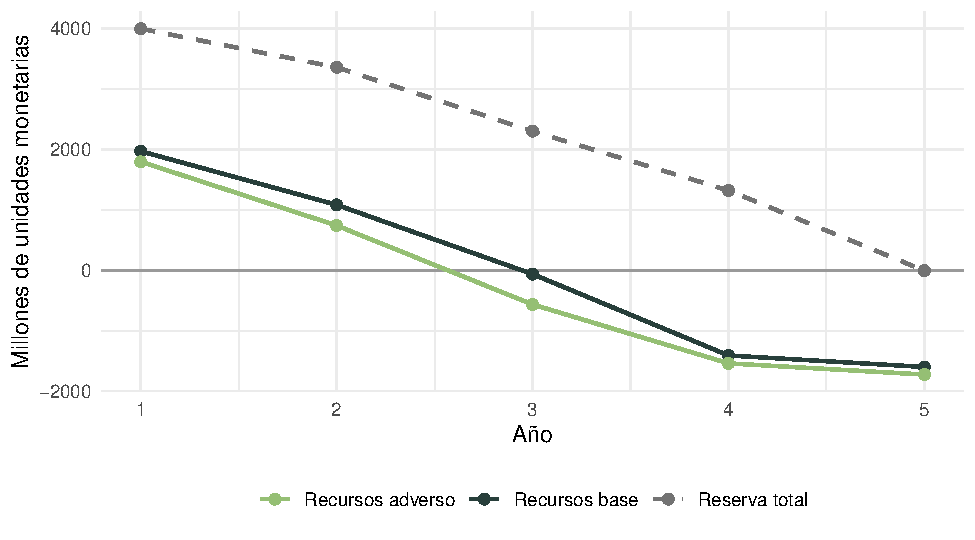
\includegraphics[width=0.85\textwidth]{recursos_vs_reserva.pdf}
\caption{Recursos antes del aporte y reserva total, por escenario (millones de unidades monetarias). Generado por \textbf{4\_escenario\_adverso.R}.}
\end{figure}

\clearpage

\section*{Anexo E. Cuenta individual \textit{equity-linked}}
\label{sec:anexo-equity}

En la trayectoria 1, el cargo del $2\%$ deja $98\,000$ para invertir y el del $3\%$ deja $97\,000$, de modo que con un rendimiento del $12{,}5344\%$ el primer año cierra en $110\,283{,}67$ y $109\,158{,}32$, respectivamente. Al cierre del quinto año, los tres saldos quedan por debajo de su garantía y el NPV es negativo en los dos casos con garantía de $110\,000$.

\begin{table}[htbp]
\centering
\small
\setlength{\tabcolsep}{4pt}
\begin{tabular}{@{}rrrrrrr@{}}
\toprule
Año & Tasa de cargo & Rendimiento & Saldo inicial & Cargo & Saldo final & VP de cargo \\
\midrule
1 & 2\% & 12,53\% & 100\,000,00 & 2\,000,00 & 110\,283,67 & 2\,000,00 \\
2 & 2\% & -11,48\% & 110\,283,67 & 2\,205,67 & 95\,669,50 & 2\,050,47 \\
3 & 2\% & 6,28\% & 95\,669,50 & 1\,913,39 & 99\,641,88 & 1\,653,39 \\
4 & 2\% & 2,77\% & 99\,641,88 & 1\,992,84 & 100\,350,34 & 1\,600,42 \\
5 & 2\% & -5,82\% & 100\,350,34 & 2\,007,01 & 92\,616,64 & 1\,497,70 \\
1 & 3\% & 12,53\% & 100\,000,00 & 3\,000,00 & 109\,158,32 & 3\,000,00 \\
2 & 3\% & -11,48\% & 109\,158,32 & 3\,274,75 & 93\,727,02 & 3\,044,32 \\
3 & 3\% & 6,28\% & 93\,727,02 & 2\,811,81 & 96\,622,63 & 2\,429,72 \\
4 & 3\% & 2,77\% & 96\,622,63 & 2\,898,68 & 96\,316,68 & 2\,327,89 \\
5 & 3\% & -5,82\% & 96\,316,68 & 2\,889,50 & 87\,986,76 & 2\,156,24 \\
\bottomrule
\end{tabular}
\caption{Saldos y cargos anuales de la trayectoria 1, en unidades monetarias, con una proyección común para ambas garantías con cargo del $2\%$.}
\label{tab:equity-trayectoria-anual}
\end{table}

\begin{table}[htbp]
\centering
\small
\begin{tabular}{@{}lrrr@{}}
\toprule
Garantía / cargo & 100\,000 / 2\% & 110\,000 / 2\% & 110\,000 / 3\% \\
\midrule
Saldo al cierre del año 5 & 92\,616,64 & 92\,616,64 & 87\,986,76 \\
Complemento al vencimiento & 7\,383,36 & 17\,383,36 & 22\,013,24 \\
VP de cargos & 8\,801,98 & 8\,801,98 & 12\,958,18 \\
VP del complemento & 5\,118,63 & 12\,051,29 & 15\,261,02 \\
NPV del proveedor & 3\,683,35 & -3\,249,31 & -2\,302,84 \\
\bottomrule
\end{tabular}
\caption{Cierre de la cuenta y NPV del proveedor en la trayectoria 1, en unidades monetarias.}
\label{tab:equity-trayectoria}
\end{table}

\begin{figure}[!htbp]
\centering
\graphicspath{{resultados/equity_linked/}}
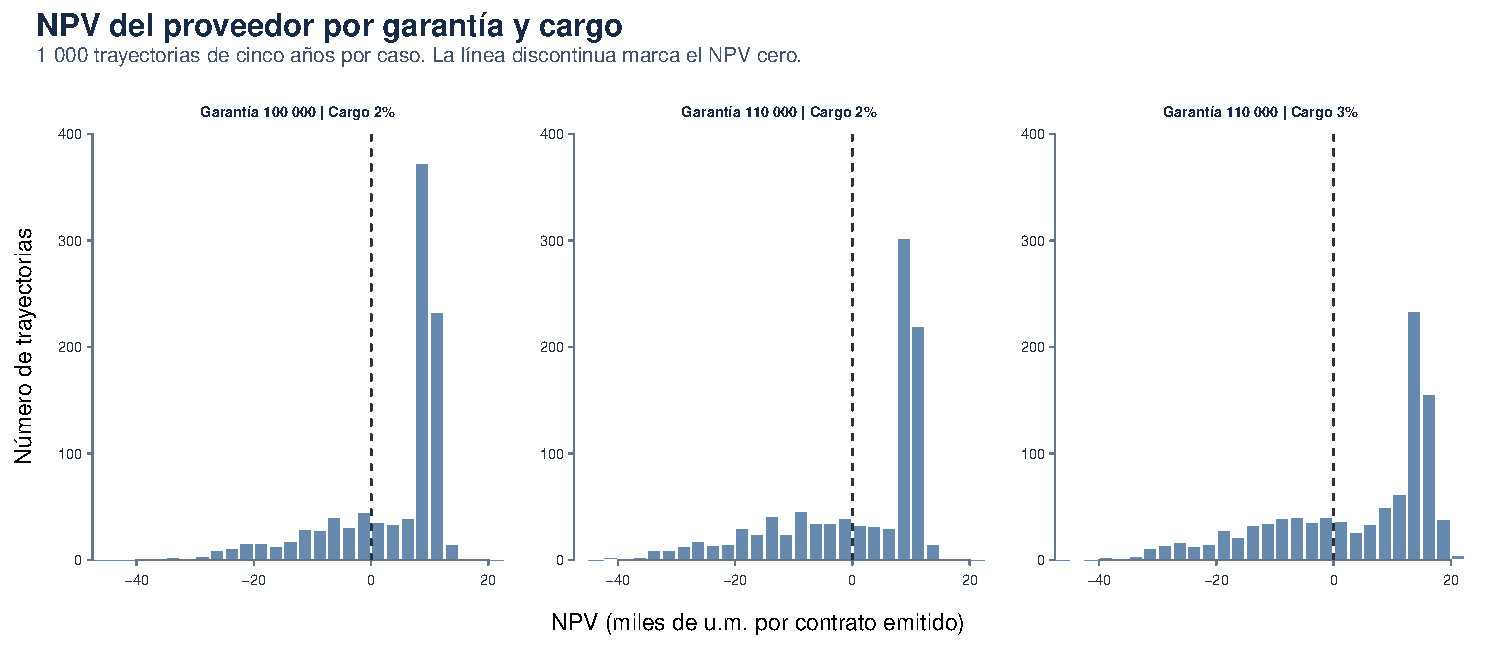
\includegraphics[width=0.95\textwidth]{histograma_npv.pdf}
\caption{Distribución del NPV por caso, con las mismas escalas e intervalos de $2\,500$ unidades monetarias.}
\label{fig:equity-npv}
\end{figure}

\end{document}

